%%%%%%%%%%%%%%%%%%%%%%%%%%%%%%%%%%%%%%%%%%%%%%%%%%%%%%%%%%%
% --------------------------------------------------------
% Rho
% LaTeX Template
% Version 2.0.0 (21/05/2024)
%
% Authors: 
% Guillermo Jimenez (memo.notess1@gmail.com)
% Eduardo Gracidas (eduardo.gracidas29@gmail.com)
% 
% License:
% Creative Commons CC BY 4.0
% --------------------------------------------------------
%%%%%%%%%%%%%%%%%%%%%%%%%%%%%%%%%%%%%%%%%%%%%%%%%%%%%%%%%%%

\documentclass[9pt,a4paper,twoside]{rho-class/rho}
\setbool{rho-abstract}{false} % Set false to hide the abstract
\setbool{corres-info}{false} % Set false to hide the corresponding author section
\setbool{linenumbers}{false} % Set false to hide the line numbering

%----------------------------------------------------------
% TITLE
%----------------------------------------------------------

\journalname{Processos Estocásticos e Vibrações Aleatórias}
\title{Trabalho}

%----------------------------------------------------------
% AUTHORS AND AFFILIATIONS
%----------------------------------------------------------

\author[1]{Leonardo Maia Nogueira}


%----------------------------------------------------------




%----------------------------------------------------------
% DATES
%----------------------------------------------------------

%\dates{This manuscript was compile on April 28, 2024}

%----------------------------------------------------------
% FOOTER INFORMATION
%----------------------------------------------------------

\leadauthor{Author last name et al.}
\footinfo{Creative Commons CC BY 4.0}
\smalltitle{\LaTeX\ Template}
\institution{College name}
\theday{May 21, 2024} %\today

%----------------------------------------------------------
% ARTICLE INFORMATION
%----------------------------------------------------------

\corres{Provide the corresponding author information and publisher here.}
\email{example@organization.com.}
\doi{\url{https://www.doi.org/exampledoi/XXXXXXXXXX}}

\received{March 20, 2024}
\revised{April 16, 2024}
\accepted{April 20, 2024}
\published{May 21, 2024}

\license{Rho LaTeX Class \ccLogo\ This document is licensed under Creative Commons CC BY 4.0.}

%----------------------------------------------------------
% ABSTRACT
%----------------------------------------------------------


%----------------------------------------------------------



%----------------------------------------------------------

\begin{document}
	
    \maketitle
    \thispagestyle{firststyle}
    % \tableofcontents

%----------------------------------------------------------

\section{Enunciado}
O artigo Hambric et al 2004, "Vibrations of plates with clamped and free edges excited by low-speed
turbulent boundary layer flow.", fornecido junto com o trabalho apresenta uma análise da resposta
vibratória de uma placa submetida a uma excitação na forma de uma camada limite turbulenta (TBL -
Turbulent Boundary Layer). O artigo examina diferentes condições de contorno para a placa e algumas
simplificações para o modelo de TBL empregado (modelo de Corcos).
De forma similar, o artigo Marcheto et al 2017, "Vibroacoustic response of panels under diffuse acousticfield excitation from sensitivity functions and reciprocityprinciples" examina a resposta vibratória de um painel submetido a uma excitação aleatória distribuída na forma de um Campo Acústico Difuso. Com base nos artigos e utilizando o código em MatLab fornecido com um modelo de placa em FEM, faça:

\begin{enumerate}
	\item  Reproduza os resultados do artigo Hambric et al 2004 para a condição analisada com uma borda livre;
	\item Calcule a resposta da placa considerada no item 1, considerando uma excitação na forma de um campo acústico difuso. Para tanto, considere a formulação para a densidade espectral cruzada fornecida no artigo Marcheto et al 2017 e o Autoespectro encontrado no item 1.
	\item Compare as resposta e discuta os resultados.
\end{enumerate}

\section{Solução}

\begin{equation}
	\Phi_{pp}(x_\mu,x_v,\omega)=\bar{\phi}_{pp}(\omega)\Gamma(\xi_1,\xi_3,\omega)
\end{equation}

\begin{equation}
	\phi_{pp}(\omega)\approx\left(\frac{\tau_w^2\delta^*}{U_0}\right)\left(\frac{5.1}{1+0.44(\omega\delta^*/U_0)^{7/3}}\right)
\end{equation}

\begin{equation}
	\mathrm{Re}_\delta\approx8U_0\delta^*/\nu, \quad \tau_w\approx0.0225\rho U_0^2/\mathrm{Re}_\delta^{0.25}
\end{equation}

\begin{figure}[H]
	\centering
	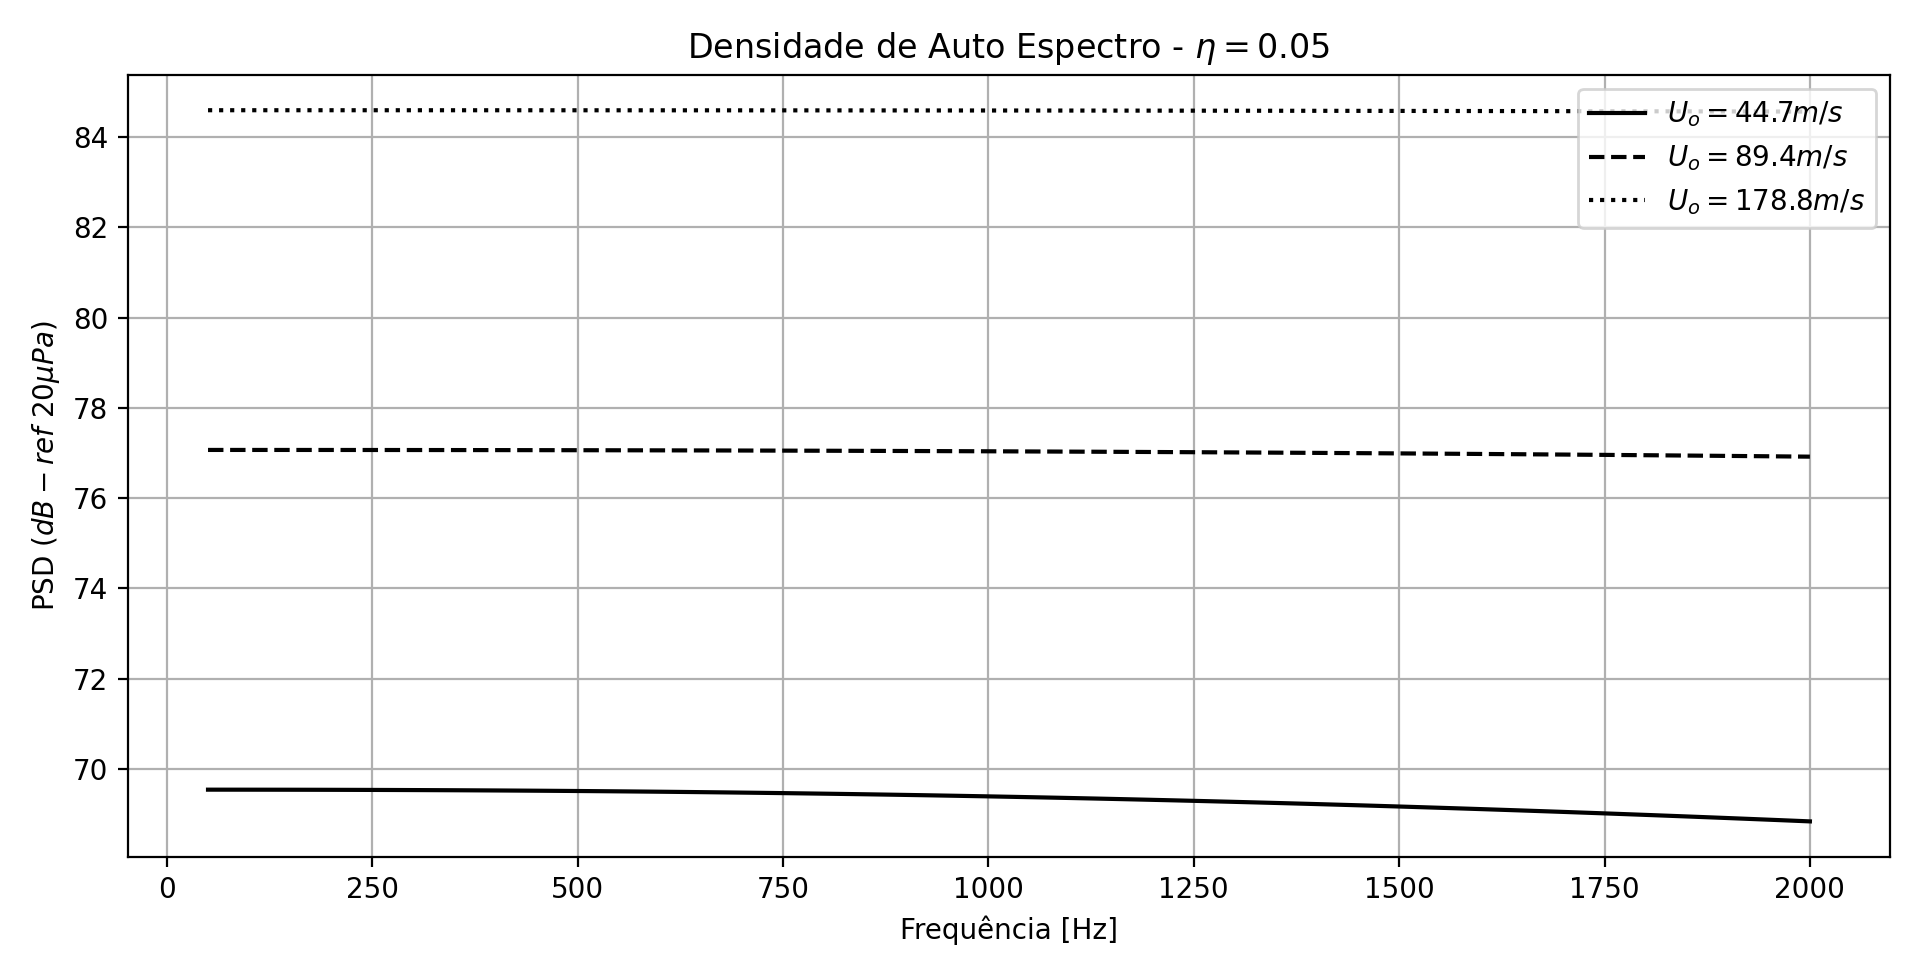
\includegraphics[width=0.9\columnwidth]{figures/psd_vel.png}
	\caption{Autoespectro de Entrada}
	\label{fig:psd}
\end{figure}

\begin{equation}
	\Gamma(\xi_1,\xi_3,\omega)=A(\omega\xi_1/U_c)B(\omega\xi_3/U_c)
\end{equation}

\begin{equation}
	U_c\cong U_0(0.59+0.30\mathrm{e}^{-0.89\omega\delta^*/U_0})
\end{equation}

\begin{eqnarray}
	A(\omega\xi_1/U_c)=(1+\alpha_1|\omega\xi_1/U_c|)\mathrm{e}^{-\alpha_1|\omega\xi_1/U_c|}\mathrm{e}^{\mathrm{i}\omega\xi_1/U_c} \\
	B(\omega\xi_3/U_c)=\mathrm{e}^{-\alpha_3|\omega\xi_3/U_c|}
\end{eqnarray}


\begin{equation}
	G_{x_\mu x_v}(\omega)=A_{x_\mu}\phi_{pp}(\omega)A_{x_v}\Gamma(\xi_1,\xi_3,\omega)
\end{equation}







\begin{figure}[H]
	\centering
	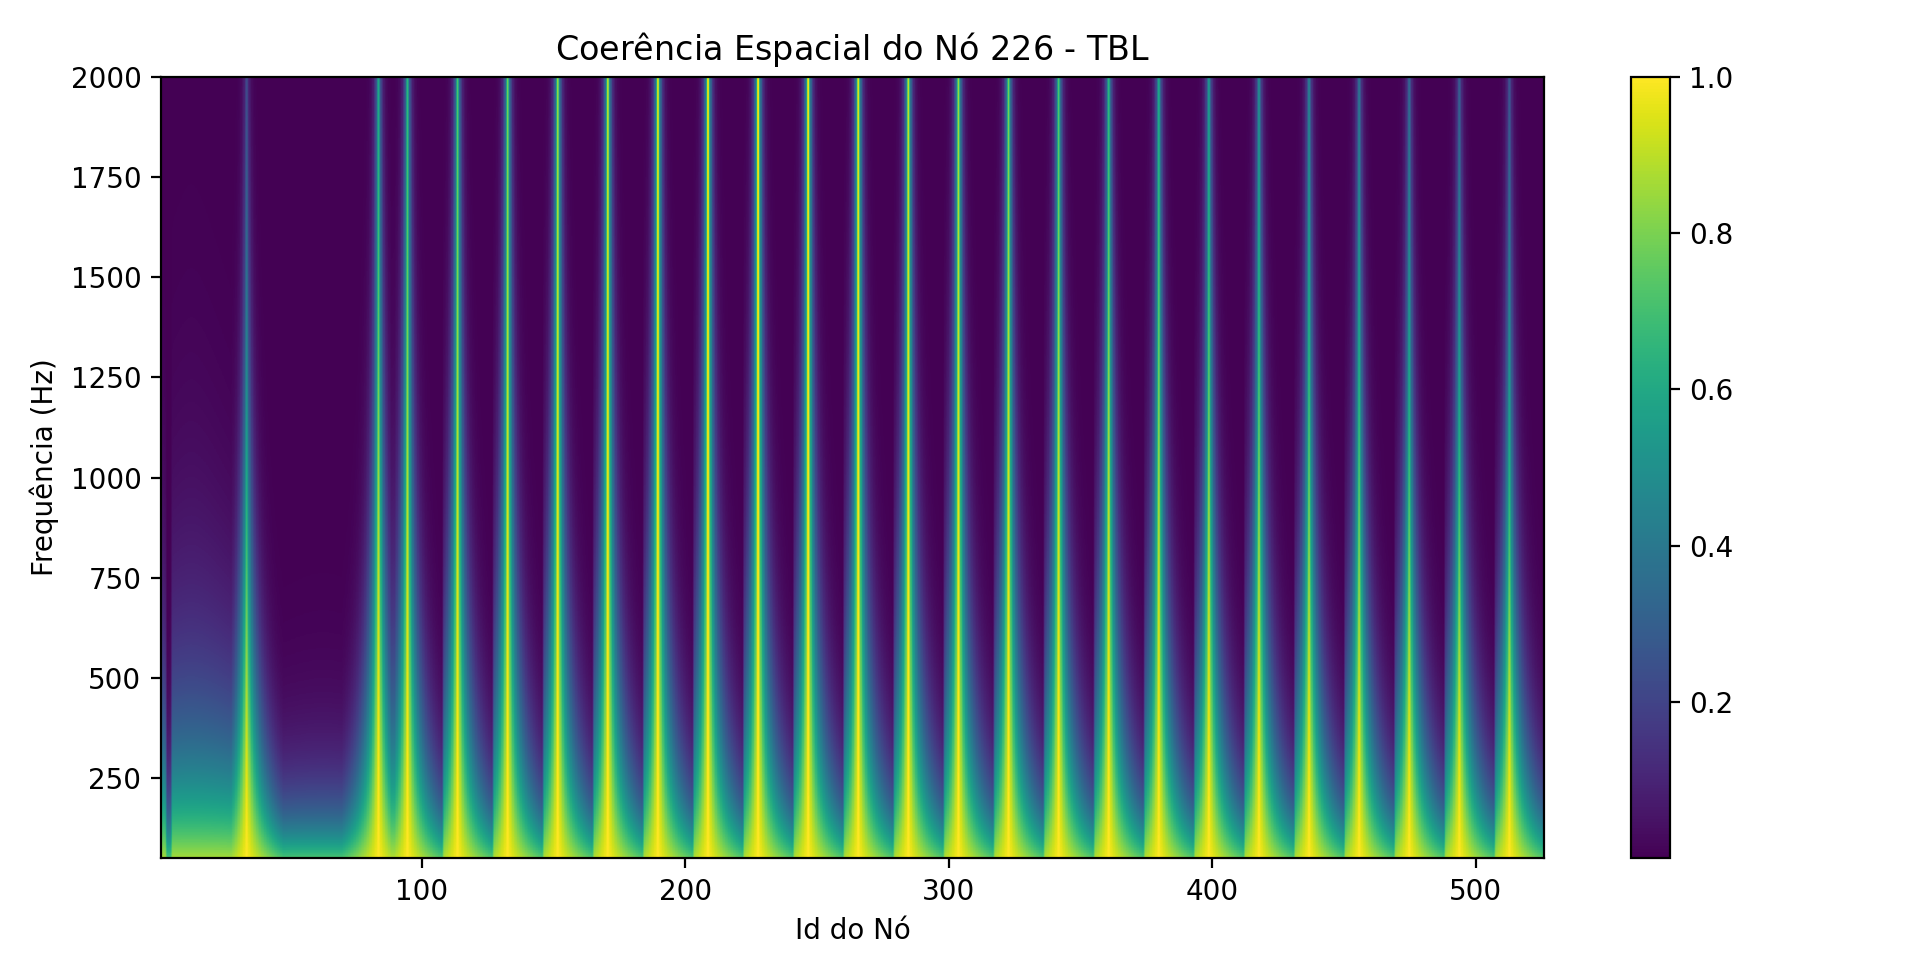
\includegraphics[width=0.9\columnwidth]{figures/coer_TBL.png}
	\caption{}
	\label{fig:coerTBL}
\end{figure}

\begin{figure}[H]
	\centering
	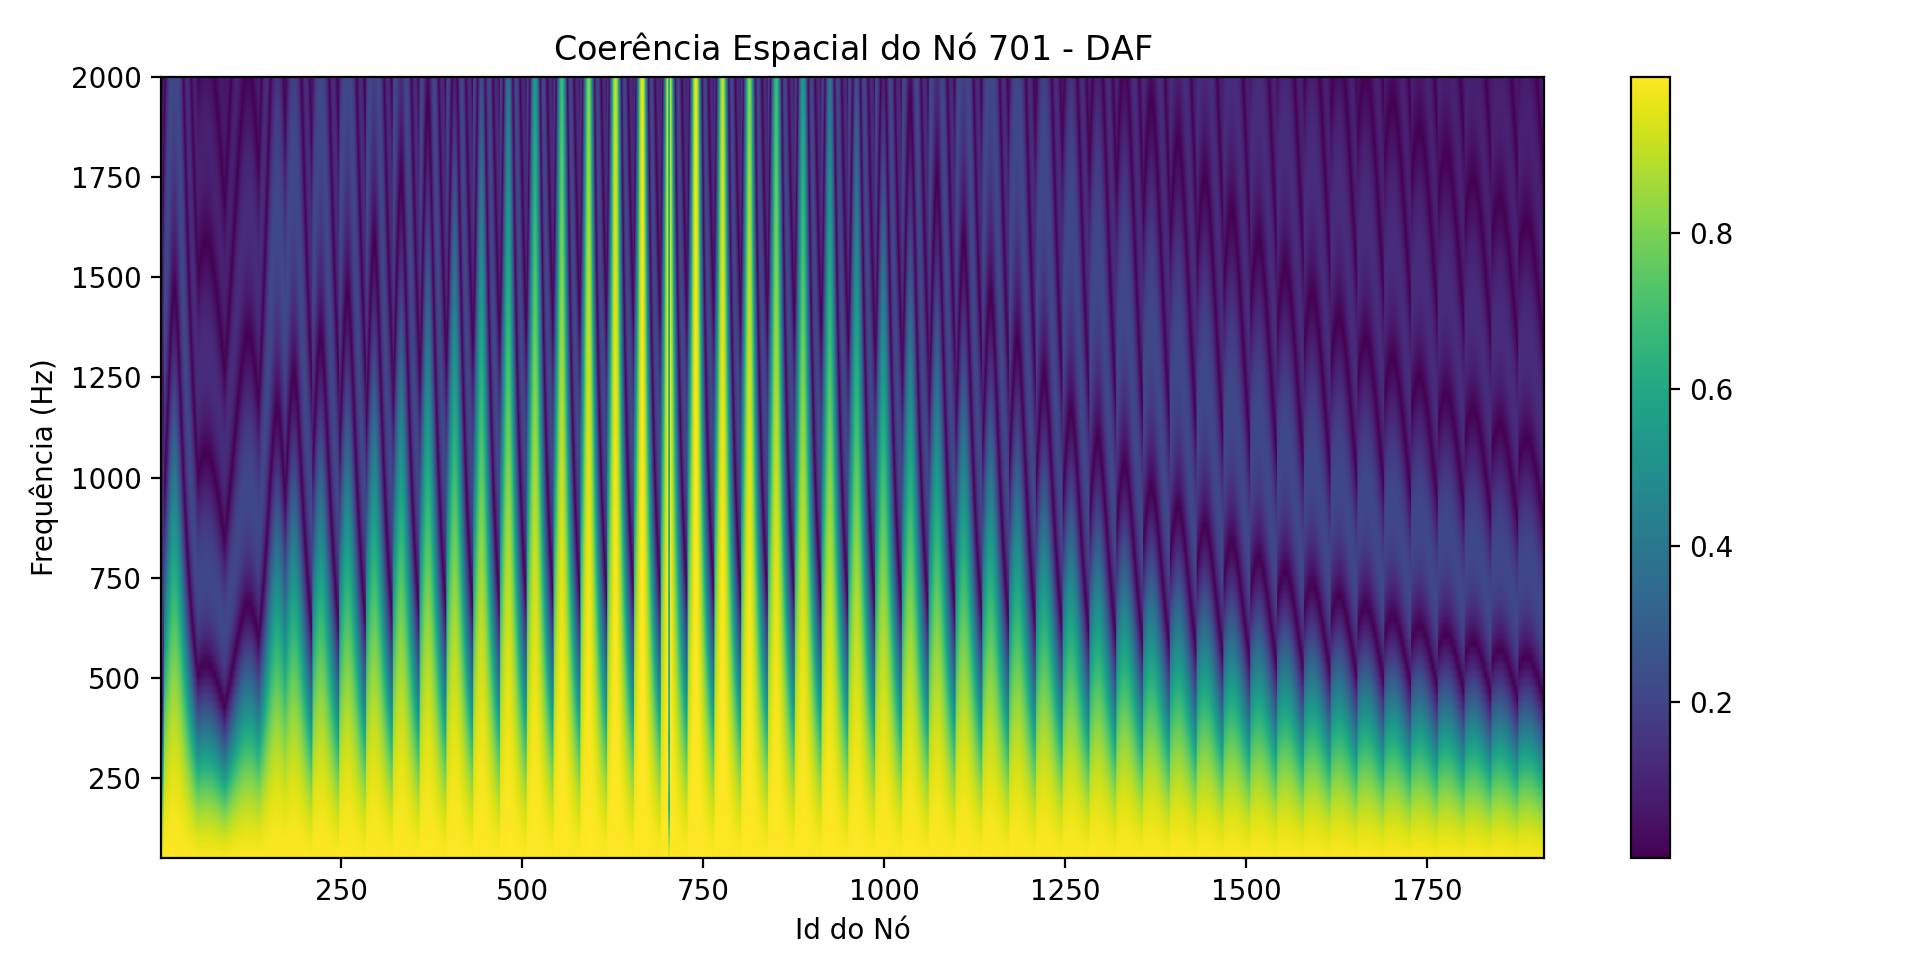
\includegraphics[width=0.9\columnwidth]{figures/coer_DAF.png}
	\caption{}
	\label{fig:coerDAF}
\end{figure}




\begin{figure}[H]
	\centering
	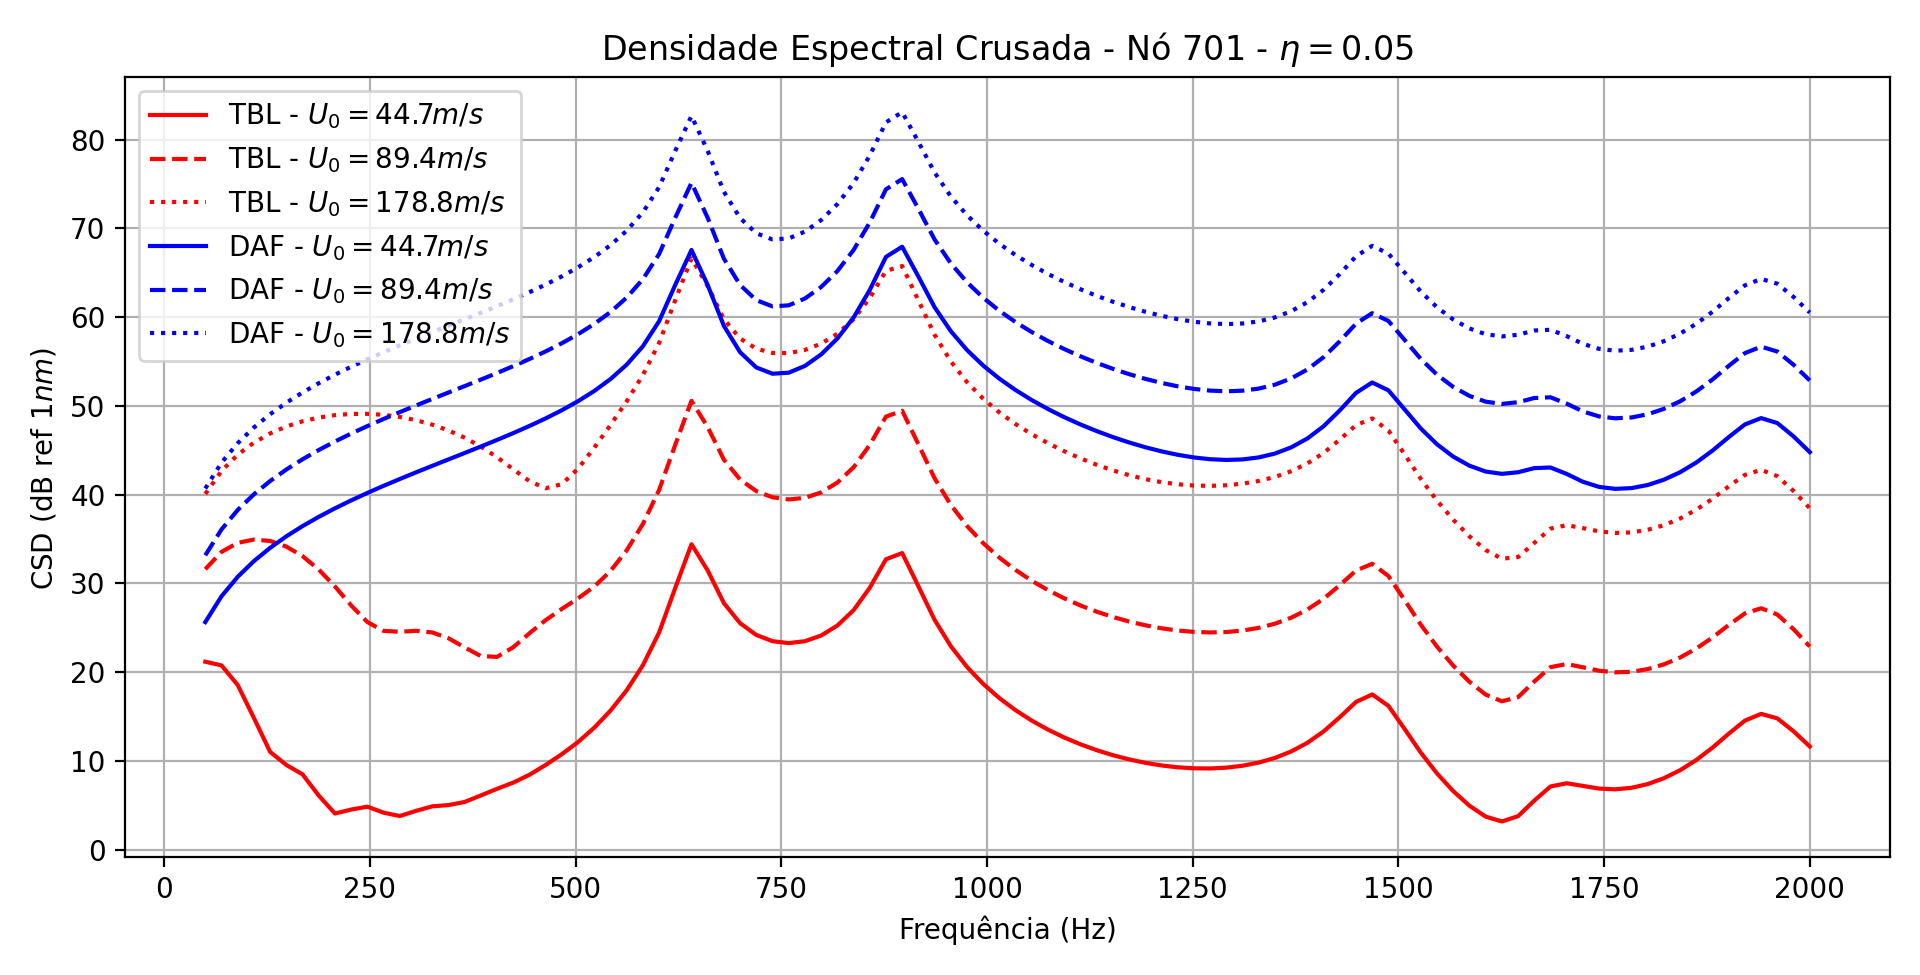
\includegraphics[width=0.9\columnwidth]{figures/csd_vel.png}
	\caption{}
	\label{fig:csdvel}
\end{figure}

\begin{figure}[H]
	\centering
	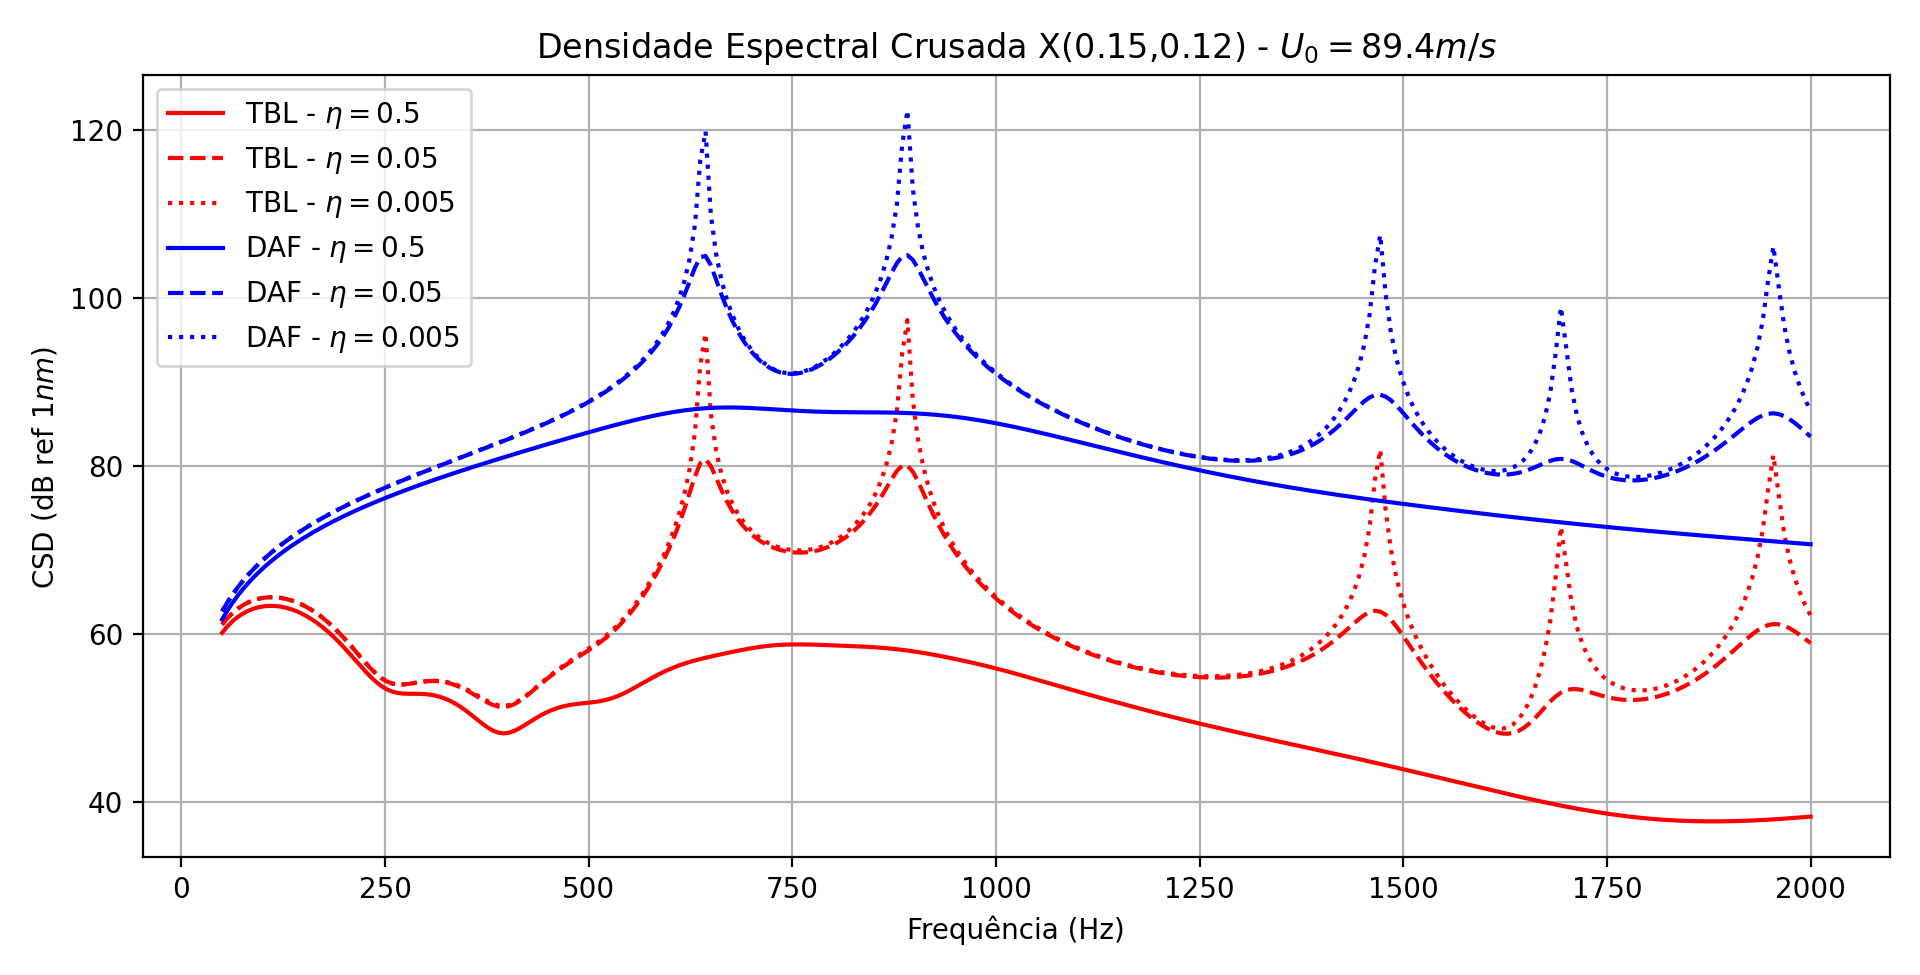
\includegraphics[width=0.9\columnwidth]{figures/csd_eta.png}
	\caption{}
	\label{fig:csdeta}
\end{figure}


%----------------------------------------------------------

\printbibliography

%----------------------------------------------------------

\end{document}